
\chapter{Marco Teórico}

Este capítulo introduce a los conceptos más relevantes para el desarrollo de este trabajo. Se abordan conceptos de Visión Artificial, Inteligencia Artificial, Aprendizaje Maquina, Aprendizaje Profundo, entre otros.
%pretende definir los conceptos usados para la realización de este trabajo de tesis.

\section{Visión artificial}

La visión artificial intenta describir el mundo que vemos en imágenes y reconstruir sus propiedades (\cite{szeliski2010computer}), con ayuda de la visión artificial es posible darle la capacidad a una máquina para identificar, analizar y procesar imágenes del mundo real. En esta sección se explicará como, una máquina representa una imagen para después representarla en una pantalla o simplemente procesarla. Por otro lado se define el filtro Kalman el cual fue utilizado para el seguimiento de objetos.

\subsection{Representación de imágenes}

En computación una imagen se representa como una cuadrícula, donde cada recuadro es llamado píxel. Un píxel es la unidad más pequeña de la imagen y representa un color (\cite{rosebrock2017deep}). Con lo anterior se entiende, que para una imagen de 1000 x 600 se tienen, 1000 píxeles en cada fila y 600 píxeles para cada columna resultando 600,000 píxeles en total. Además, son dos las representaciones más comunes de un píxel (i.e escala de grises, color).

%\begin{itemize}
%\item Escala de grises
%\item A color
%\end{itemize}

Cuando se representa una imagen utilizando escala de grises cada píxel tiene un valor numérico en el rango de 0 a 255. Con este rango de valores es posible variar la intensidad de color presentado, siendo 0 el valor para representar el color negro y 255 el color blanco. Teniendo esto en cuenta se puede interpretar que los valores intermedios son diferentes intensidades de grises, de ahí el nombre escala de grises.

Para los píxeles a color existen diferentes espacios de colores, en este trabajo solo se hablara acerca del espacio de color RGB. Los píxeles RGB son representados usando 3 valores de intensidad para los colores rojo, verde y azul. Cada uno de estos 3 valores tiene un rango del 0 al 255 con lo cual se pueden variar los colores presentados. Al igual que la escala de grises cada uno de estos 3 valores pueden tener valores en el intervalo de 0 a 255. Al colocar los 3 valores de RGB a '0' (cero) se representa el color negro, por el contrario, para representar el color blanco los 3 valores de RGB deben ser de 255.

Ahora bien, para el caso de la representación de los videos, estos se pueden representar utilizando escala de grises o a color. Ya que los videos son una secuencia de imágenes con las cuales se genera la sensación de movimiento. Para el caso de los videos, al conjunto de imágenes que forman el video se les llama fotogramas y pueden variar en su frecuencia. A la frecuencia de imágenes contenidas en un tiempo determinado se le conoce como fotogramas por segundo. Hoy en día los fotogramas por segundo más comunes son 60, sin embargo, ya hay implementaciones con una mayor cantidad.
La resolución tanto de una imagen como de un video se establece por la cantidad de píxeles en el eje X y el eje Y. Existen diferentes resoluciones de las cuales la más común es \textit{Full HD}, en la Tabla \ref{tab:resolutions} se muestra el resto de las resoluciones más comunes.

\begin{table}[H]
    \caption{Resoluciones de video}
    \centering
    \label{tab:resolutions}
    \begin{tabular}{|c|c|c|}
    \hline
    \textbf{SIGLAS} & \textbf{NOMBRE} & \textbf{RESOLUCIÓN} \\ \hline
    \textbf{SD}     & \textit{Standard Definition} & 640 x 480 píxeles \\ \hline
    \textbf{QHD}    & \textit{Quarter of High Definition} & 960 x 540 píxeles \\ \hline
    \textbf{HD}     & \textit{High Definition} & 1.280 x 720 píxeles \\ \hline
    \textbf{FHD}    & \textit{Full HD o Full High Definition} & 1.920 x 1.080 píxeles \\ \hline
    \textbf{QHD}    & \textit{Quad High Definition} & 2.560 x 1.440 píxeles \\ \hline
    \textbf{UHD}    & \textit{Ultra High Definition} & 3.840 x 2.160 píxeles \\ \hline
    \end{tabular}
\end{table}

\subsection{Filtro Kalman}

El filtro Kalman es una solución recursiva al filtrado lineal de datos discretos (\cite{welch1995introduction}). Se encarga de estimar las variables de estado en un sistema dinámico, lo cual, en el caso del presente trabajo, implica estimar la siguiente ubicación de un vehículo identificado.

El filtro de Kalman tiene como objetivo resolver el problema general de estimar el estado $x \space \epsilon \space \mathbb{R} ^{n}$ de un proceso controlado en tiempo discreto, el cual se representa con la Ecuación \ref{eq:kalmanEstado}.

La matriz $A$  de dimensión $n\times{}n$ en la Ecuación \ref{eq:kalmanEstado} relaciona el estado en el paso de tiempo $k$ con el estado en el paso $k + 1$, en ausencia de una función de excitación o ruido de proceso. La matriz $B$ de dimensión $n\times{}1$ relaciona la entrada de control $u \space \epsilon \mathbb{R}^{1}$ con el estado $x$. La matriz $H$ de dimensión $m\times{}n$ en la ecuación de medición ( Ecuación \ref{eq:kalmanMed}) relaciona el estado con la medición $z_k$.

\begin{equation}
\label{eq:kalmanEstado}
    x_{k+1} = A_kx_k + Bu_k + w_k
\end{equation}
\myequations{Filtro Kalman. Ecuación de estado}

Con una medida $z \space \epsilon \space \mathbb{R}^{m}$:

\begin{equation}
\label{eq:kalmanMed}
    z_x = H_kx_k + v_k
\end{equation}
\myequations{Filtro Kalman. Relación estado y medición}

Las variables $w_k$ y $v_k$ representan el error del proceso y de la medida respectivamente.

El algoritmo de filtro Kalman cuenta con dos fases, la fase predicción (a priori) y la fase de corrección (a posteriori), según se aprecia en la Figura \ref{fig:AlgoritmoFiltroKalman}.

\begin{figure}[H]
    \centering
    \begin{tikzpicture}
    \node (a)[rectangle , draw=black, minimum height=4.5cm,
        text width=5.5cm]{
        \centering
        \textbf{Predicción}
        \\~\\
        \raggedright
        Predicción \\
        $\bar{x}_{k+1} = A_k\hat{x}_k + Bu_k$ \\
        Predicción covarianza del error \\
        $P_{k+1} = A_kP_kTA^{T}_k + Q_k$
    };

    \node (b)[rectangle , draw=black, minimum height=4.5cm,
        text width=5.5cm]
        [right=3cm of a]
    {
        \centering
        \textbf{Corrección}
        \\~\\
        \raggedright
        Cálculo ganancia de Kalman \\
        $K_k = P_kH^{T}_k(H_kP_KH^{T}_k + R_k)$ \\
        Actualiza la estimación \\
        $\hat{x}_k = \hat{x}_k + K(z_k - H_k \hat{x}_k)$ \\
        Actualiza covarianza del error \\
        $P_k = (I - K_kH_k)P_k$
    };
    
    \draw[->, very thick] (a.north) .. controls +(up:1.8cm) and +(up:1.8cm) .. (b.north);
    \draw[->, very thick] (b.south) .. controls +(down:1.8cm) and +(down:1.8cm) .. (a.south);
    
    \end{tikzpicture}
    \caption{Algoritmo filtro Kalman (\cite{welch1995introduction}).}
    \label{fig:AlgoritmoFiltroKalman}
\end{figure}

Para la fase de predicción se toman las Ecuaciones \ref{eq:kalmanActUno} y \ref{eq:kalmanActDos}:

\begin{eqnarray}
    \label{eq:kalmanActUno}
    \bar{x}_{k+1} = A_k\hat{x}_k + Bu_k\\
    \label{eq:kalmanActDos}
    P_{k+1} = A_kP_kTA^{T}_k + Q_k
\end{eqnarray}

Las ecuaciones anteriores, pronostican el estado y la covarianza desde $k$ hasta $k+1$. La matriz $A$ representa el estado actual. $Q$ representa la covarianza de la perturbación aleatoria del proceso.

La fase de corrección cuenta con las Ecuaciones \ref{eq:kalmanCorrUno}, \ref{eq:kalmanCorrDos} y \ref{eq:kalmanCorrTres}:

\begin{eqnarray}
    \label{eq:kalmanCorrUno}
    K_k = P_kH^{T}_k(H_kP_KH^{T}_k + R_k)\\
    \label{eq:kalmanCorrDos}
    \hat{x}_k = \hat{x}_k + K(z_k - H_k \hat{x}_k)\\
    \label{eq:kalmanCorrTres}
    P_k = (I - K_kH_k)P_k
\end{eqnarray}

La Ecuación \ref{eq:kalmanCorrUno} representa el primer pasa el cual es el cálculo de ganancia de Kalman, $K_t$. El siguiente paso es medir el proceso para obtener $z$, y luego generar una estimación del estado a posteriori incorporando la medición como en la Ecuación \ref{eq:kalmanCorrDos}. El último paso es obtener una estimación de la covarianza del error a posteriori mediante la Ecuación \ref{eq:kalmanCorrTres}.

Después de cada actualización y medición, el proceso se repite con las estimaciones a posteriori anteriores utilizadas para proyectar o predecir las nuevas estimaciones a priori.


\section{Inteligencia Artificial}

\subsection{Historia}

El comienzo de las redes neuronales comienza en la década de 1940 con el artículo de Warren McCulloch y Walter Pitts \cite{mcculloch1943Logical}, con el cual demostraron que es posible calcular cualquier función aritmética o lógica con el uso de redes neuronales artificiales.

En 1950 Frank Rosenblatt \cite{rosenblatt1958Perceptron} crea la red perceptrón, la cual es conocida como la primera aplicación práctica de las redes neuronales. Rosenblatt construyo una red perceptrón capaz de reconocer patrones. Lo cual dio inicio a la investigación del campo de las redes neuronales. No obstante, tiempo después Minsky and Papert \cite{minsky1969Perceptrons} demostraron que la red perceptrón solo podía resolver ciertos problemas específicos.

Con la publicación de Minsky and Papert muchos investigadores creyeron que no tenía sentido continuar con las redes neuronales. Además, de la limitante computacional de la época para realizar los experimentos que se requerían. Lo cual llevo a una pausa para la investigación de las redes neuronales por una década.

En la década de 1980 David Rumelhart y James McClelland \cite{rumelhart1986Parallel} crean el algoritmo de Backpropagation para el entrenamiento de las redes perceptrón multicapa, lo cual marca el renacimiento de las redes neuronales. Este algoritmo fue la respuesta al libro de Minsky y Papert de 1960.

\section{Aprendizaje Maquina}
\label{sec:MachineLearning}

La inteligencia artificial incorpora un conjunto diverso de trabajos relacionados con el razonamiento automático mientras que el subcampo del aprendizaje maquina se especializa en el reconocimiento de patrones y el aprendizaje de los datos (\cite{rosebrock2017deep}).

El aprendizaje maquina utiliza algoritmos para extraer información o patrones de un conjunto de datos(\textit{Dataset}) sin procesar y representarla en un modelo, después usar este modelo para inferir resultados sobre otros datos que aún no hemos modelado (\cite{patterson2017deep}).

El aprendizaje maquina utiliza estadísticas.Tradicionalmente se resuelve un problema determinista en el que nuestra solución resuelve el problema todo el tiempo. Hay muchos problemas en los que la solución no es determinista. Es decir, no sabemos lo suficiente sobre el problema o no tenemos suficiente potencia para modelar correctamente el problema. Para estos problemas necesitamos estadísticas(\cite{harrington2012Machine}).

En otras palabras, el aprendizaje maquina es un subcampo de la inteligencia artificial, este se encarga de aprender los patrones con los cuales podemos modelar un conjunto de datos, una vez aprendido los patrones más importantes se crea un modelo que podemos utilizar para identificar cierto conjunto de datos.

La metodología utilizada en el aprendizaje maquina es relativamente sencilla, por ejemplo, si queremos aprender a identificar si una imagen contiene un animal como un ratón o un gato, debemos tomar cierto número de muestras(cientos o miles). Con estas muestras el aprendizaje maquina se encargará de tomarlas y procesarlas para identificar las caracterizas más importantes, estas características son el modelo que define a cada animal. Ahora bien, podemos tomar una de las muestras y pasarla por el modelo creado, con esto es muy probable que el modelo nos diga correctamente que animal esta la imagen, es por esto que se utilizan muestras que no hayan sido procesadas anteriormente.

La RAE define aprender como adquirir el conocimiento de algo por medio del estudio o de la experiencia, en nuestro caso la maquina aprende por medio de la experiencia adquirida al procesar cada una de las muestras, a tal grado que identifica muestras que no estaban en el conjunto de datos de entrada. En aprendizaje maquina se le llama entrenamiento al proceso de generación de un modelo a partir de las muestras, mientras que la validación es el proceso con el cual el modelo infiere resultados a partir de muestras que no pasaron por el proceso de entrenamiento. El conjunto de datos son todas las muestras que serán utilizadas para el proceso de entrenamiento y validación.

Comúnmente el conjunto de datos es dividido para cada proceso, entrenamiento y validación, en la práctica lo más común es separar el conjunto de un porcentaje de 70-30, siendo 70\% para el proceso de entrenamiento y 30\% para la validación.

Mas adelante se presentan las métricas que se utilizan para evaluar el modelo por medio del conjunto de datos de validación. En el aprendizaje maquina tenemos tres tipos diferentes de aprendizaje: aprendizaje supervisado, aprendizaje no supervisado y aprendizaje semi-supervisado, a continuación, se describen los tres tipos de aprendizaje, sin embargo, en este trabajo solo se hablará con más detalle sobre el aprendizaje supervisado.

\begin{itemize}

    \item Aprendizaje supervisado: Es un proceso de entrenamiento en el que se realizan predicciones sobre los datos de entrada y luego se corrigen las predicciones incorrectas. El proceso continúa hasta que se obtiene un error bajo o un número máximo de iteraciones. Para esto es necesario que nuestros datos de entrada tengan cierta etiqueta con el significado de cada uno de nuestros datos.

    \item Aprendizaje no supervisado: En este aprendizaje no tenemos nuestros datos con la etiqueta correspondiente a su valor. Para este caso es el entrenamiento el encargado de encontrar cierto patrón en los datos con el cual asignara una etiqueta a cada uno de ellos.

    \item Aprendizaje semi-supervisado: En el aprendizaje semi-supervisado tenemos datos etiquetados y datos sin etiquetar. El proceso de entrenamiento toma los datos conocidos, los analiza y etiqueta cada uno de los datos no etiquetados para usarlos como datos de entrenamiento adicionales. El algoritmo semi-supervisado aprende la “estructura" de los datos.

\end{itemize}


\subsection{Aprendizaje supervisado}

En la Sección \ref{sec:MachineLearning} menciono un poco sobre el aprendizaje supervisado, ahora vamos a hablar sobre dos tipos de problemas que nos podemos encontrar al resolverlos utilizando aprendizaje máquina.

\subsubsection{Clasificación}

En el aprendizaje maquina la clasificación consiste en que el algoritmo aprenda los patrones que definen un conjunto de datos perteneciente a una clase especifica. Los valores de salida del modelo es la categoría correspondiente a los datos de entrada que pueden ser dos o más opciones bien definidas.

La clasificación binaria es la forma más simple de clasificación en esta se tienen solo dos valores de salida (0 o 1). Esta clasificación nos sirve para responder a la simple pregunta si pertenece o no a una clase en concreto. Por ejemplo, podemos identificar si una transacción bancaria es fraudulenta o no.

Existen una gran variedad de conjuntos de datos con una gran cantidad de clases como MNIST, Animals, CIFAR-10, Flowers-17 entre otros cada uno de estos son útiles para validar el correcto funcionamiento de una red neuronal.

\begin{figure}[H]
    \centering
    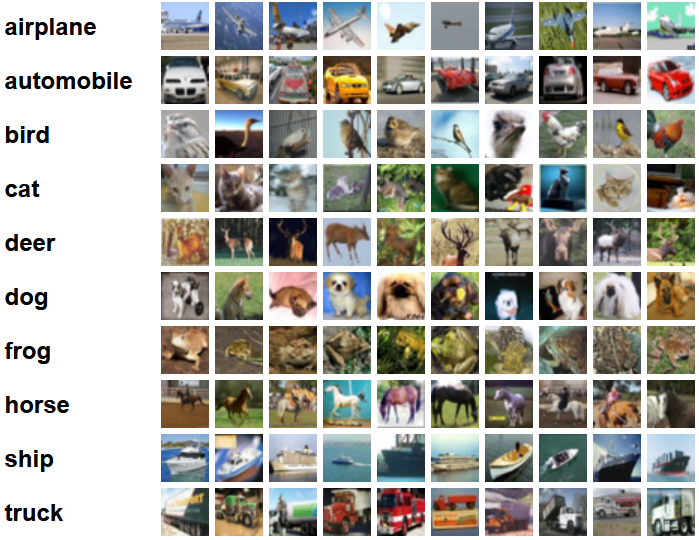
\includegraphics[width=0.6\textwidth]{MarcoTeorico/imgs/CIFAR-10.png}
    \caption{\textit{Dataset} CIFAR-10.}
    \label{fig:cifar10}
\end{figure}

Para todo aquel problema que implique separar un conjunto de datos en diferentes clases o categorías, sin importar el numero clases que pueden ser, se utiliza la clasificación.

\subsubsection{Regresión}

Los problemas de regresión predicen un valor real. En otras palabras, la función que estima la variable dependiente conociendo la variable independiente.

La regresión es utilizada para aquellos problemas que implican predecir valores numéricos, un ejemplo de esto son las predicciones de ráfagas de vientos las cuales dando como entrada diferentes características del ambiente podemos predecir la velocidad del viento.

\subsubsection{Regresión Lineal}

La clase más común de regresión es la regresión lineal. La regresión lineal intenta llegar a una función que describa la relación entre $x$ y $y$, para valores conocidos de $x$, predice valores de $y$ que resultan ser precisos (\cite{patterson2017deep}). La Figura \ref{fig:regresionLineal} representa la regresión en una gráfica.

\begin{figure}[H]
    \centering
    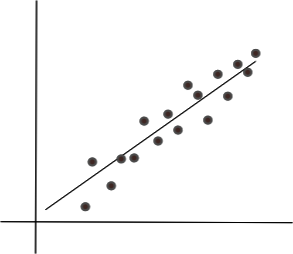
\includegraphics[width=0.5\textwidth]{MarcoTeorico/imgs/RegresionLineal.png}
    \caption{Grafica de regresión lineal.}
    \label{fig:regresionLineal}
\end{figure}

\subsubsection{Regresión Ridge}

La regresión Ridge es una versión regularizada de la regresión lineal, agrega un término de regularización en la función de costo (Ecuación \ref{eq:ridge}). Con esto se busca que el algoritmo mantenga los pesos lo más pequeños posible.

\begin{equation}
    \label{eq:ridge}
    \alpha \displaystyle\sum\limits_{i=1}^n (\theta_i)^{2}
\end{equation}

El hiperparametro $\alpha$ controla la regularización del modelo, si $\alpha = 0$ la regresión Ridge es simplemente una regresión lineal. Si $\alpha$ es muy grande, todos los pesos terminan igual a cero y resulta en una línea plana que pasa por la media de los datos(Figura \ref{fig:regresionRidge}.

\begin{figure}[H]
    \centering
    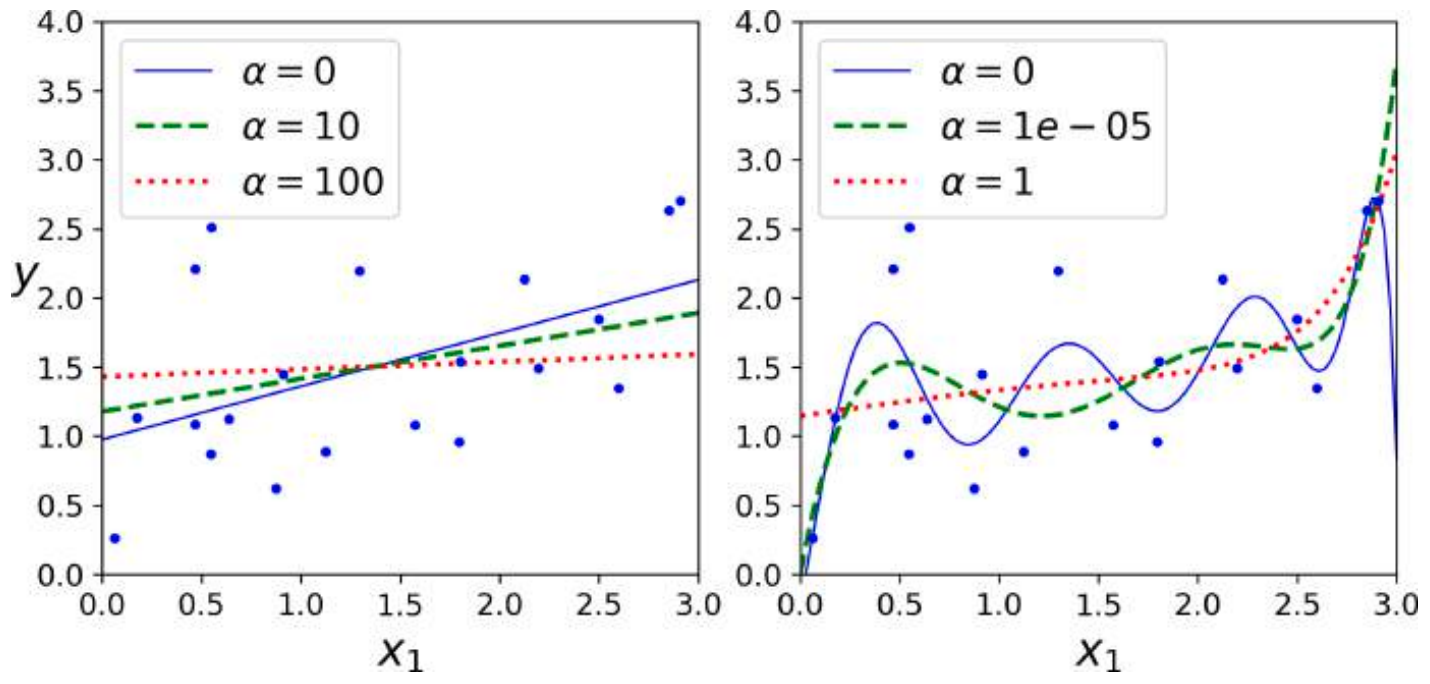
\includegraphics[width=0.8\textwidth]{MarcoTeorico/imgs/Ridge.png}
    \caption{Regresión Ridge con diferentes valores de $\alpha$.}
    \label{fig:regresionRidge}
\end{figure}

La Ecuación \ref{eq:ridgeCostFunction} es la función de costo para la regresión Ridge.

\begin{equation}
    \label{eq:ridgeCostFunction}
    J(\theta) = MSE(\theta)
    + \alpha \displaystyle\sum\limits_{i=1}^n (\theta_i)^{2}
\end{equation}

\subsubsection{Regresión Lasso}

La regresión Lasso (\textit{Least Absolute Shrinkage and Selection Operator} en Ingles) al igual que la regresión Ridge es una versión regularizada de la regresión lineal, sin embargo, la regresión Lasso utilizada valores absolutos en la función de regulación (Ecuación \ref{eq:lasso}), una característica importante con Lasso es que puede llegar a eliminar por completo los pesos de las características menos importantes.

\begin{equation}
    \label{eq:lasso}
    \alpha \displaystyle\sum\limits_{i=1}^n  \mid \theta_i \mid
\end{equation}

La Ecuación \ref{eq:lassoCostFunction} es la función de costo para la regresión Lasso.

\begin{equation}
    \label{eq:lassoCostFunction}
    J(\theta) = MSE(\theta)
    + \alpha \displaystyle\sum\limits_{i=1}^n  \mid \theta_i \mid
\end{equation}

\subsubsection{Elastic Net}

Elastic Net es una versión regularizada de la regresión lineal, siendo el punto medio entre la regresión Ridge y Lasso, utiliza un valor de regularización $r$, cuando $r = 0$ Elastic Net es equivalente a Ridge, y cuando $r = 1$, se comporta como Lasso (Ecuación \ref{eq:elasticNet}).

\begin{equation}
    \label{eq:elasticNet}
    r \alpha \displaystyle\sum\limits_{i=1}^n  \mid \theta_i \mid
    + \frac{1 - r}{2} \alpha \displaystyle\sum\limits_{i=1}^n  (\theta_i)^{2}
\end{equation}

La Ecuación \ref{eq:elasticNetCostFunction} es la función de costo para la regresión Elastic Net.

\begin{equation}
    \label{eq:elasticNetCostFunction}
    J(\theta) = MSE(\theta)
    + r \alpha \displaystyle\sum\limits_{i=1}^n  \mid \theta_i \mid
    + \frac{1 - r}{2} \alpha \displaystyle\sum\limits_{i=1}^n  (\theta_i)^{2}
\end{equation}

\subsection{Sobreajuste y Subajuste}

Cuando es entrenado un nuevo modelo se busca que tenga la capacidad de generalizar de tal manera que pueda interpretar datos de entrada que nunca haya visto.

Un buen modelo se equivoca poco en sus predicciones, esto significa que tiene un error bajo. Esto se evalúa ingresando al modelo datos que no recibió en su proceso de entrenamiento, de esta manera se tiene la seguridad de que el modelo es capaz de generalizar.

El subajuste ocurre cuando el modelo no puede obtener una pérdida suficientemente baja en el conjunto de entrenamiento. En este caso, el modelo no aprende los patrones en los datos de entrenamiento. Lo cual implica una gran cantidad de errores cuando es utilizado para realizar predicciones, como muestra la Figura \ref{fig:OverFiting}.


\begin{figure}[H]
    \centering
    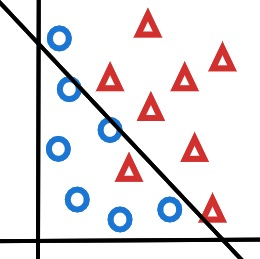
\includegraphics[width=0.4\textwidth]{MarcoTeorico/imgs/Ajuste_subajuste.jpg}
    \caption{Ejemplo de subajuste.}
    \label{fig:OverFiting}
\end{figure}


Por otro lado, tenemos un sobreajuste cuando la red modela los datos de entrenamiento demasiado bien y no se generaliza a los datos de validación (\cite{rosebrock2017deep}). En este caso tenemos que las predicciones solo serán buenas para aquellos que se utilice el mismo conjunto de datos que en el entrenamiento, Figura \ref{fig:underFiting}.

\begin{figure}[H]
    \centering
    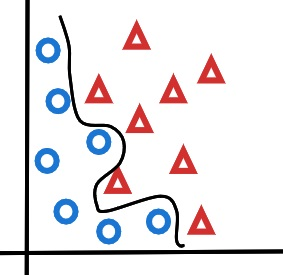
\includegraphics[width=0.4\textwidth]{MarcoTeorico/imgs/Ajuste_sobreajuste.jpg}
    \caption{Ejemplo de sobreajuste.}
    \label{fig:underFiting}
\end{figure}

Por otra parte, el entrenamiento ideal es cuando la red modela los datos de entrenamiento con cierto margen de error, pero siendo su gran mayoría correcta, Figura \ref{fig:idealFiting}.

\begin{figure}[H]
    \centering
    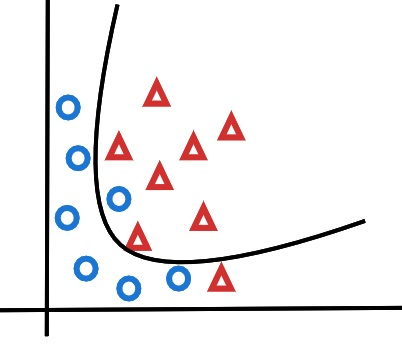
\includegraphics[width=0.6\textwidth]{MarcoTeorico/imgs/Ajuste_ideal.jpg}
    \caption{Ejemplo de ideal.}
    \label{fig:idealFiting}
\end{figure}

\subsection{Métricas de evaluación}


Ahora bien, cuando se realiza el entrenamiento es necesario saber que tan bueno es el modelo que se ha generado, para esto existen diferentes métricas que nos indican de manera cuantitativa la calidad del modelo.

Cuando se ha entrenado un modelo para un problema de clasificación se utilizan medidas de exactitud como una métrica de evaluación. La exactitud se calcula con el número de predicciones correctas entre el número de predicciones totales, La Ecuación \ref{eq:exactitud} muestra la métrica de exactitud.

\begin{equation}
    \label{eq:exactitud}
    Exactitud = \frac{Predicciones \: correctas}{ Total \: de \: predicciones}
\end{equation}

Por otra parte, los modelos creados para problemas de regresión hay tres métricas principales MAE, MSE Y RMSE.

La métrica de evaluación del Error Absoluto Medio (MAE – \textit{Mean Absolute Error} en Ingles) calcula la media de los valores absolutos de la diferencia entre los valores reales y los predichos. En otras palabras, MAE es el promedio de todos los errores sin tomar en cuenta si este error es positivo o negativo con respecto al valor real. La Ecuación \ref{eq:MAE} define el calculo de MAE.

\begin{equation}
    \label{eq:MAE}
    MAE = (\frac{1}{n}) \displaystyle\sum\limits_{i=0}^n \mid y_i - x_i \mid
\end{equation}

El Error Medio Cuadrado (MSE – \textit{Mean Square Error} en Ingles) se encarga de elevar al cuadrado el error, penalizando fuertemente los valores que se alejan demasiado del valor real esperado, con este valor se obtiene el promedio, la Ecuación \ref{eq:MSE} define el calculo de MSE.

\begin{equation}
    \label{eq:MSE}
    MSE = (\frac{1}{n}) \displaystyle\sum\limits_{i=0}^n (y_i - x_i)^{2}
\end{equation}

La Raíz del Error Cuadrático Medio (RMSE – \textit{Root Mean Square Error} en Ingles) al igual que la métrica MSE penaliza los errores altos, solo que para esta métrica se eliminan los cuadrados obteniendo la raíz del promedio obtenido con MSE. La Ecuación \ref{eq:RMSE} define el calculo de RMSE.

\begin{equation}
    \label{eq:RMSE}
    RMSE = \sqrt {
        (\frac{1}{n}) \displaystyle\sum\limits_{i=0}^n (y_i - x_i)^{2}
    }
\end{equation}

\section{Aprendizaje profundo}

\subsection{Redes neuronales}

Una red neuronal se llama así porque los científicos intentaron modelar el cerebro en código informático. El objetivo final es crear una “inteligencia general artificial”, en otras palabras un programa que puede aprender todo lo que una persona podria aprender.

Las redes neuronales artificiales son una clase de algoritmos de aprendizaje máquina que aprenden de los datos y se especializan en el reconocimiento de patrones (\cite{rosebrock2017deep}).

Una red neuronal es una función flexible que adapta de manera autónoma su comportamiento para satisfacer la relación entre la entradas y los resultados esperados y se ha denominado como un aproximador universal (\cite{goyal2018Deep}).

\subsection{Perceptrón}

Rosenblatt publicó el algoritmo seminal Perceptron: este modelo podía aprender automáticamente los pesos necesarios para clasificar una entrada.

Perceptron toma n entradas y produce una única salida binaria si la suma es mayor que el valor de activación. Se dice que la neurona se "dispara" siempre que se excede el valor de activación y se comporta como una función escalonada, lo cual se muestra en la ecuación \ref{eq:fnStep} (\cite{goyal2018Deep}).

\begin{equation}
\label{eq:fnStep}
    f\left(x\right)=\begin{cases}0 & x -u < 0\\1 & x -u >= 0\end{cases}
\end{equation}



Minsky y Papert demostraron que un perceptrón con una función de activación lineal es simplemente un clasificador lineal, incapaz de resolver problemas no lineales (\cite{rosebrock2017deep}). El ejemplo canónico de un problema no lineal es el conjunto de datos XOR Figura \ref{fig:xor}.

Perceptron se puede convertir fácilmente en un algoritmo en línea que procesa un flujo de ejemplos, actualizando el vector de peso solo si el último ejemplo recibido está mal clasificado. Se garantiza que el perceptrón convergerá en una solución si los datos de entrenamiento son linealmente separables, pero de lo contrario no convergerán(\cite{flach2012Machine}).

\begin{figure}[H]
    \centering
    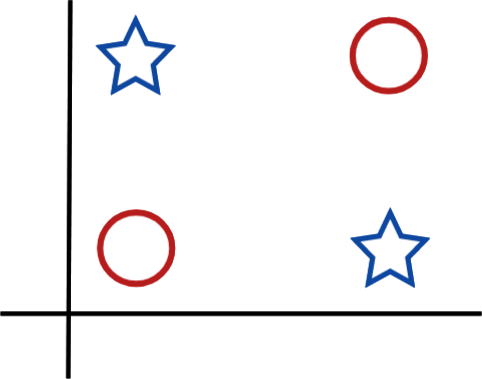
\includegraphics[width=0.5\textwidth]{MarcoTeorico/imgs/XOR.png}
    \caption{Problema XOR, no es linealmente separable.}
    \label{fig:xor}
\end{figure}


\subsection{Redes Neuronales Multicapa}


Los perceptrones multicapa o MLP (Multilayer Perceptron) son una red neuronal de propagación hacia adelante y se componen de múltiples perceptrones conectados entre sí y que operan en funciones de activación distintivas para permitir mejores mecanismos de aprendizaje. La arquitectura perceptrón multicapa cuenta como mínimo con 3 capas: una capa de entrada, una o más capas ocultas y una capa de salida (\cite{swamynathan2017Mastering}) Figura \ref{fig:mlp}.

\begin{figure}[H]
    \centering
    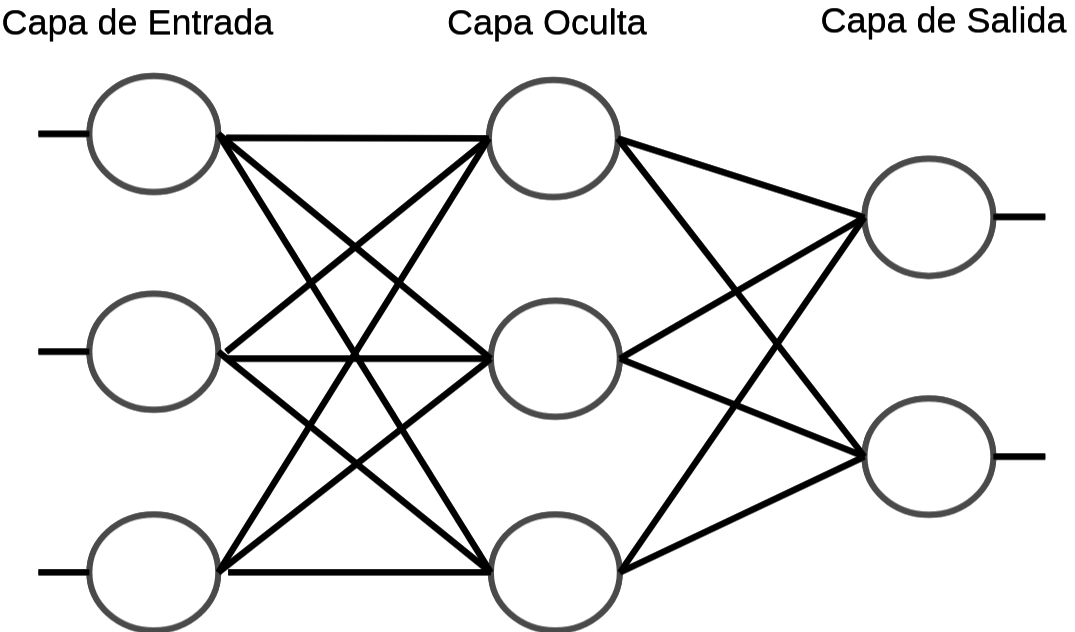
\includegraphics[width=0.5\textwidth]{MarcoTeorico/imgs/MLP.png}
    \caption{Representación básica de red neuronal multicapa.}
    \label{fig:mlp}
\end{figure}

Los MLP también se conocen como aproximadores universales, ya que pueden encontrar la relación entre los valores de entrada y los objetivos, utilizando una cantidad suficiente de neuronas en la capa oculta, alterando los pesos o utilizando datos de entrenamiento adicionales para aproximar la función dada hasta cualquier nivel de precisión. A menudo, con el grado de libertad dado a un MLP, puede superar a la red MLP básica, introduciendo más capas ocultas, con menos neuronas en cada una de las capas ocultas y pesos óptimos. Esto ayuda en el proceso de generalización general del modelo (\cite{goyal2018Deep}).

\subsection{Propagación hacia atrás(Backpropagation)}

En las redes neuronales es complicado ajustar sus pesos de entrenamiento por la gran cantidad de conexiones y sus múltiples niveles. Para lograr esta tarea, se utiliza el algoritmo backpropagation, creado por \citeauthor{rumelhart1986Parallel} en \citeyear{rumelhart1986Parallel}.

En el algoritmo Backpropagation calculamos qué tan rápido cambia el error a medida que cambiamos una capa oculta. A partir de ahí, podemos averiguar qué tan rápido cambia el error cuando cambiamos el peso de una conexión individual. Básicamente, intentamos encontrar el camino de descenso más empinado. Comenzamos calculando las derivadas del error con respecto a un solo ejemplo de entrenamiento. Una vez que tenemos las derivadas de error para una capa de unidades ocultas, las usaremos para calcular las derivadas de error para las unidades de la capa siguiente. Y una vez que encontramos las derivadas del error para las actividades de las unidades ocultas, es bastante fácil obtener las derivadas del error para los pesos que conducen a una unidad oculta (\cite{buduma2017Fundamentals}).

En resumen, el algoritmo backpropagation consiste en dos pasos como muestra la figura:

\begin{itemize}
\item Propagación hacia adelante: Se calculan los pesos de cada una de las neuronas, desde la capa de entrada hasta la capa de salida.

\item Propagación hacia atrás: Se calcula el error y se actualizan los pesos, desde la capa de salida hasta la capa de entrada.
\end{itemize}

\begin{figure}[H]
    \centering
    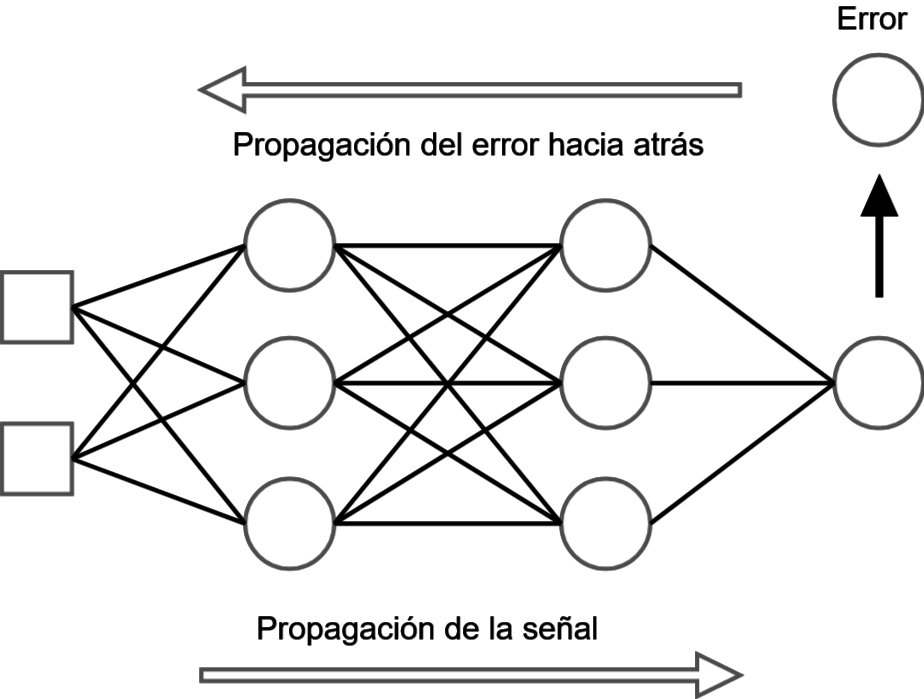
\includegraphics[width=0.8\textwidth]{MarcoTeorico/imgs/Backpropagation.png}
    \caption{Propagación hacia adelante y propagación hacia atrás.}
    \label{fig:backpropagation}
\end{figure}

\subsection{Descenso del Gradiente }

El método del descenso del gradiente es un algoritmo iterativo que minimiza una función de pérdida actualizando posteriormente los parámetros de la función.

\begin{figure}[H]
    \centering
    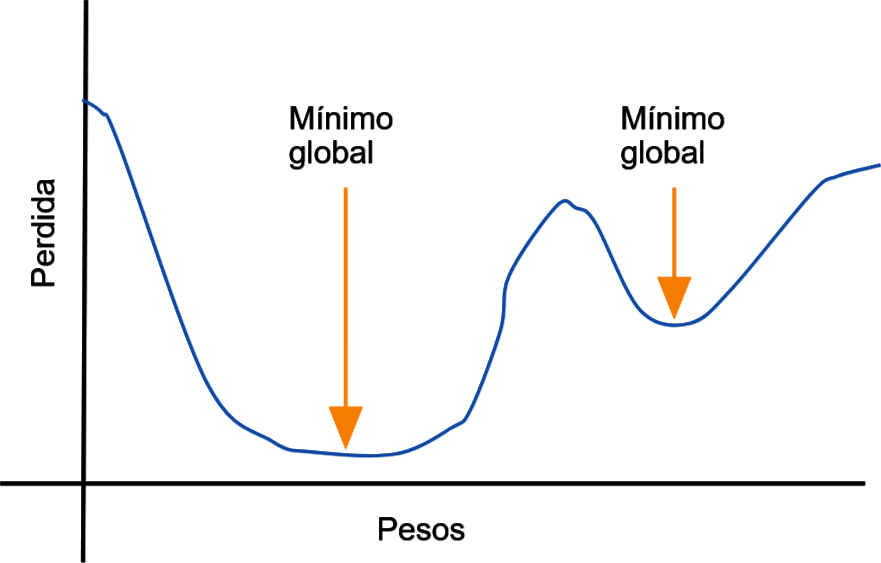
\includegraphics[width=0.8\textwidth]{MarcoTeorico/imgs/DescensoGradiente.png}
    \caption{Mínimo local y global.}
    \label{fig:descensoGradiente}
\end{figure}

La Figura \ref{fig:descensoGradiente} muestra cómo podemos tener múltiples picos y valles (Máximos y mínimos) para nuestros valores de perdida. El valor ideal que nos gustaría obtener es nuestro mínimo global, asegurando que nuestros parámetros tomen los valores más óptimos posibles.

El problema es que no tenemos una vista general en la que podamos encontrar de manera sencilla el mínimo global ya que en realidad nos colocaríamos en un lugar aleatorio sin saber dónde está el mínimo global y tendríamos que avanzar hacia una perdida mínima sin subir accidentalmente a la cima de un máximo local.

\subsection{Tasa de aprendizaje}

La tasa de aprendizaje es uno de los hiperparámetros más importantes. Tiene un fuerte impacto tanto en la estabilidad como en la eficiencia de los tiempos de entrenamiento y no hay una forma fija de encontrar la más adecuada. La tasa de aprendizaje es la magnitud del ajuste de pesos durante el entrenamiento de la red con el fin de minimizar el error (\cite{valenzuela2020Sistema}).

La imagen muestra que si la tasa es demasiado grande, nuestro entrenamiento es inestable. Si nuestra tasa de aprendizaje es demasiado pequeña, el entrenamiento puede tomar más tiempo para llegar a un entrenamiento adecuado.

\begin{figure}[H]
    \centering
    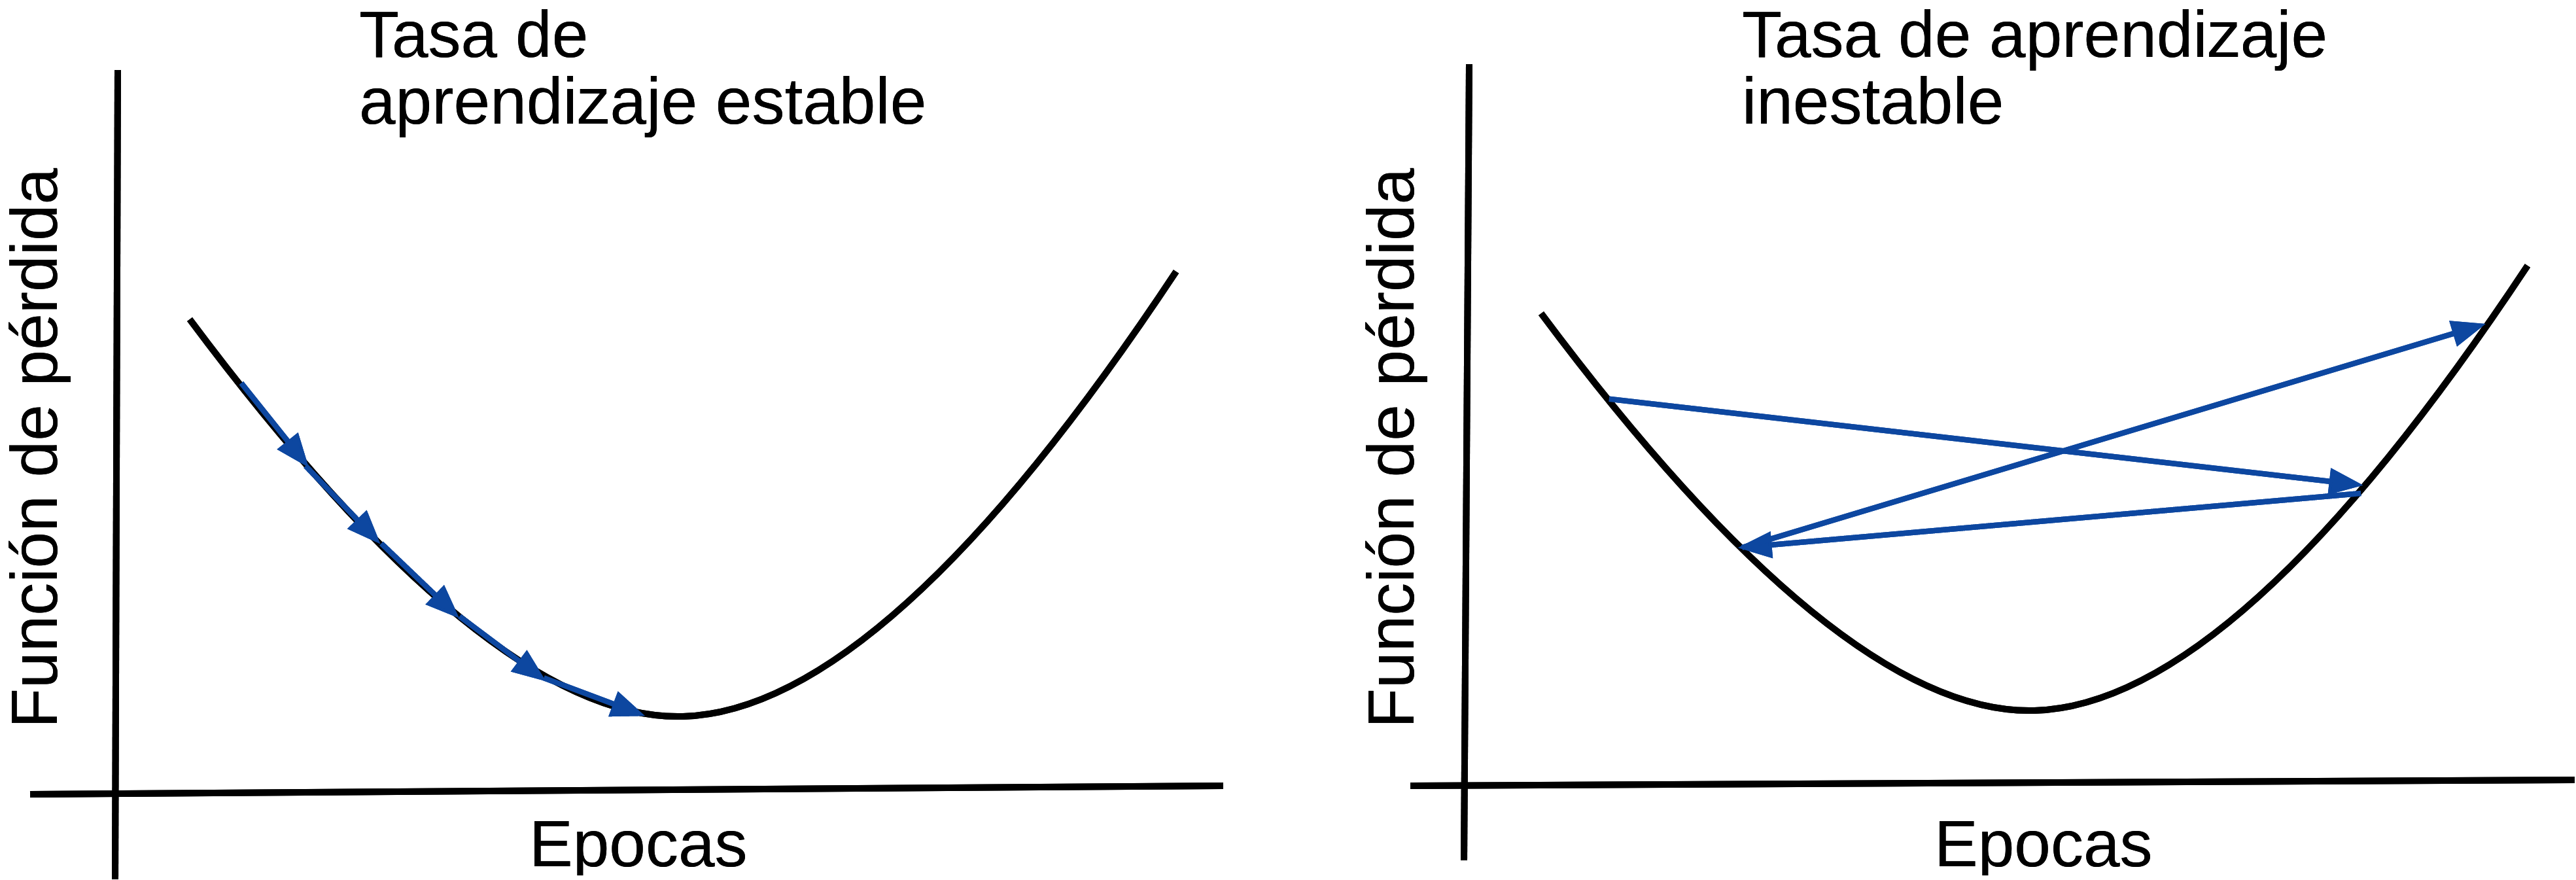
\includegraphics[width=0.8\textwidth]{MarcoTeorico/imgs/LearningRate.png}
    \caption{Tasa de aprendizaje.}
    \label{fig:learningRate}
\end{figure}

Preferiblemente, nuestra pérdida de entrenamiento y validación casi se imitan entre sí, con solo una pequeña brecha entre la pérdida de entrenamiento y la pérdida de validación, lo que indica un pequeño sobreajuste. Siempre que la brecha no aumente drásticamente, sabemos que existe un nivel aceptable de sobreajuste. Por otro lado, si no logramos mantener esta brecha y las pérdidas de entrenamiento y validación se separan drásticamente, entonces sabemos que corremos el riesgo de sobreajuste. Una vez que la pérdida de validación comienza a aumentar, sabemos que estamos muy sobreajustados (\cite{rosebrock2017deep}).


\subsection{Funciones de activación}

Las funciones de activación son una función de escalar a escalar, que produce la activación de la neurona. Usamos funciones de activación para propagar la salida de los nodos de una capa hacia la siguiente capa y para que las neuronas ocultas en una red neuronal para introducir la no linealidad del modelado de la red (\cite{patterson2017deep}).


Las funciones de activación definen el rango de valores que dará como resultado una de las capas de nuestra red neuronal, a partir de una función matemática.

\subsubsection{Función lineal}

La función lineal regresa como salida valores en el rango de $[-\infty,\infty]$ y está dada por la ecuación \ref{eq:linealFunc}:

\begin{equation}
\label{eq:linealFunc}
    f(x) = Wx
\end{equation}

\subsubsection{Sigmoidal}

La función sigmoidal nos da como salida valores en el rango de $[0,1]$ y está definida por la ecuación \ref{eq:sigmoidFunc}:

\begin{equation}
\label{eq:sigmoidFunc}
    s(x)={\frac {1}{1+e^{-x}}}
\end{equation}

\subsubsection{Tangente hiperbólica}

La función tangente hiperbólica proporciona como salida el rango $[-1,1]$ y está definida por la ecuación \ref{eq:tanhFunc}.

\begin{equation}
\label{eq:tanhFunc}
    \tanh (x)={\cfrac {e^{x}-e^{-x}}{e^{x}+e^{-x}}}
\end{equation}

\subsubsection{Softmax}

La función de activación softmax devuelve la distribución de probabilidad sobre clases de salida mutuamente excluyentes. La cual está definida por la siguiente ecuación \ref{eq:softmaxFunc}:

\begin{equation}
\label{eq:softmaxFunc}
  \sigma(\overrightarrow{z})_{i}=\frac{e^{z_{i}}}{
    \displaystyle\sum\limits_{j=1}^K e^{z_{j}}
  }
\end{equation}

donde $\overrightarrow{z}$ es el vector de entrada.

$z_i$ son los valores del vector de entrada.

$e^{z_{i}}$ es la función exponencial estándar que se aplica a cada elemento del vector de entrada.

$\displaystyle\sum\limits_{j=1}^K e^{z_{i}}$ es el término de normalización, asegura que todos los valores de salida de la función sumen 1 y cada uno esté en el rango $(0, 1)$, constituyendo así una distribución de probabilidad válida.

$k$ el numero de clases del clasificador multi-clases.

\subsubsection{ReLU}

La funcion Rectificador Lineal(ReLU) regresa como resultado valores en el rango de los números reales positivos $[0, \infty]$, como muestra la ecuación \ref{eq:reluFunc}:

\begin{equation}
\label{eq:reluFunc}
  relu(x)=\max(0,x)
\end{equation}


\subsection{Funciones de perdida}

Una función de pérdida indica la pérdida de predicción de $\hat{y}$ cuando la salida real es $y$. El objetivo del entrenamiento es entonces minimizar la pérdida en los diferentes ejemplos de entrenamiento. La función asigna una puntuación numérica a la salida de la red $\hat{y}$ dada la verdadera salida esperada $y$ (\cite{goldberg2017Neural}).

Dependiendo de nuestro problema es el tipo de función de perdida que usaremos. Para un problema de regresión se busca tener la perdida lo más cercana a cero y para un problema un problema de clasificación se busca tener el valor más algo o muy cercano a 1 para cada una de las clases para la cual fue entrenada nuestra red neuronal, siempre cuidando que la red neuronal no tenga sobreajuste claro.

Algunas de las funciones de perdida para problemas de  regresion son las siguientes:

\begin{itemize}
    \item Perdida de error cuadrático medio(MSE, \textit{Mean squared error loss})
    \item Perdida del error absoluto medio(MAE, \textit{Mean absolute error loss})
\end{itemize}

Mientras que para problemas de clasificación algunas de las funciones de perdida son las siguientes:

\begin{itemize}
    \item Perdida de bisagra
    \item Perdida logística
\end{itemize}

\subsection{Optimizadores}


\section{Tecnologías Utilizadas}

Para el desarrollo de este trabajo se utilizaron múltiples herramientas como lo son Git, SublimeText 3, Sublime Merge y los repositorios de Github todo bajo el sistema operativo Ubuntu 20.04.

A continuacion se presentan las herramientas de software de mayor impacto para el desarrollo de este trabajo.

\subsection{Python}

Python es un lenguaje de programación de alto nivel, interpretado y multipropósito. Python es muy utilizado por  la comunidad al ser un leguaje muy fácil de aprender y utilizar por ser un lenguaje de tipado dinámico, además de ser de código abierto.

Python ha tomado popularidad para el desarrollo en deep learning, por su facilidad de uso y la gran variedad de bibliotecas con las que cuenta como TensorFlow, PyTorch, Numpy, Scikit, entre otros.

\subsection{Contenedores Docker}

Un contenedor es una unidad de software que empaqueta el código y todas sus dependencias para que la aplicación se ejecute de forma rápida y confiable de un entorno informático a otro. Una imagen de contenedor de Docker es un paquete de software ligero, independiente y ejecutable que incluye todo lo necesario para ejecutar una aplicación: código, tiempo de ejecución, herramientas del sistema, bibliotecas del sistema y configuraciones \cite{docker2021container}.

La Figura \ref{fig:contenedorDocker} muestra las capas desde la infraestructura hasta los contenendores ejecutandose.

\begin{figure}[H]
    \centering
    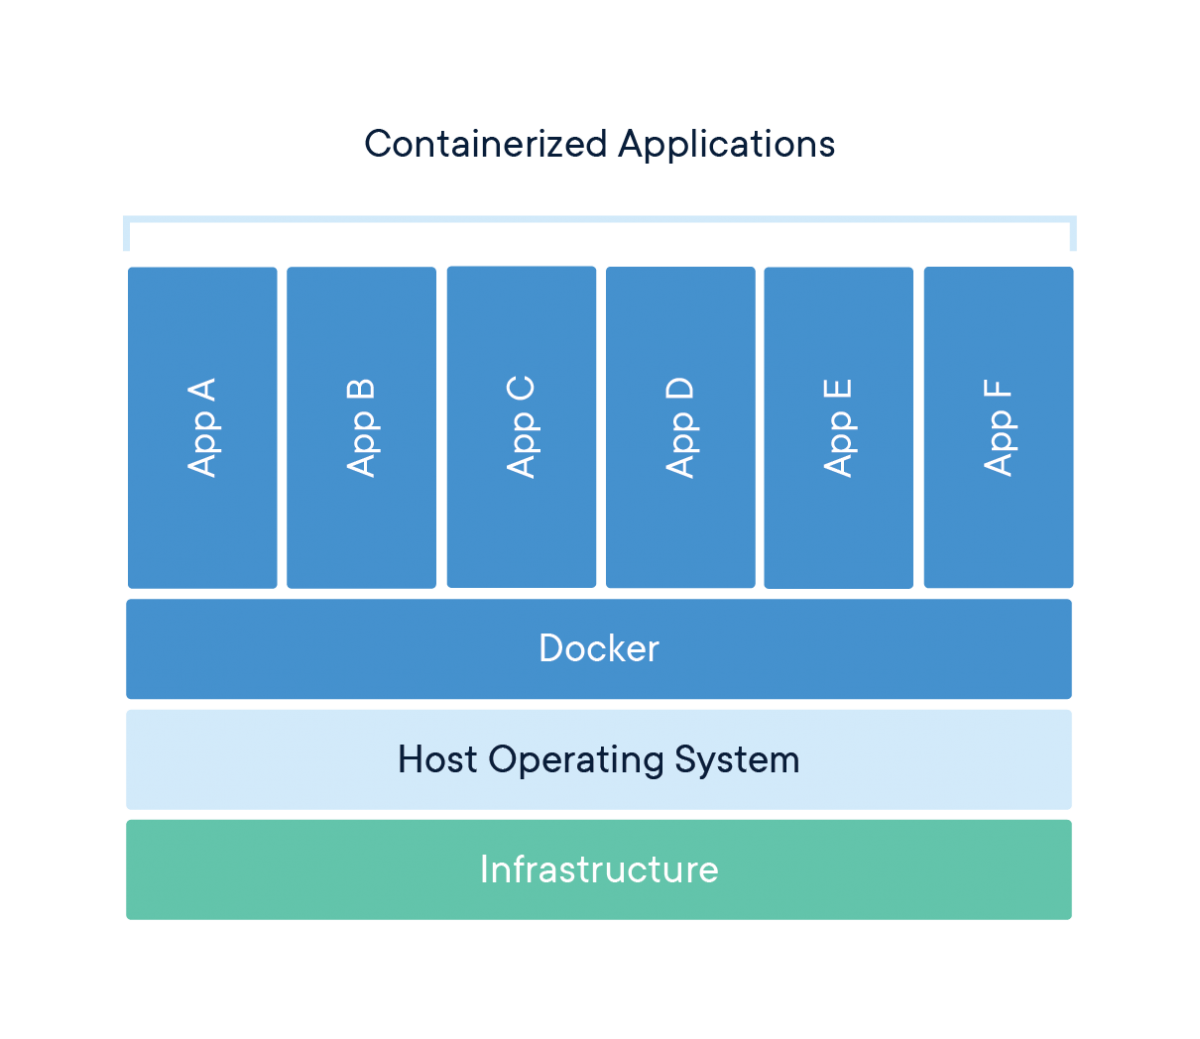
\includegraphics[width=0.6\textwidth]{MarcoTeorico/imgs/container-what-is-container.png}
    \caption{Representacion de un contenedor \cite{docker2021container}.}
    \label{fig:contenedorDocker}
\end{figure}


Docker fue la principal herramienta utilizada para el desarrollo de este trabajo, puesto que, sirvió para replicar múltiples trabajos del estado del arte sin necesidad de complicadas configuraciones al equipo utilizado, además de transferir los experimentos a otro equipo al solo utilizar la imagen creada para este experimento.

\subsection{Nvidia Docker}

NVIDIA Container Toolkit permite crear y ejecutar contenedores acelerados por GPU. Incluye una biblioteca de tiempo de ejecución de contenedores y utilidades para configurar automáticamente los contenedores para aprovechar las GPU de NVIDIA \cite{nvidiaDocker2021overview}.

Nvidia Docker permite la comunicación entre los contenedores de Docker y las GPU de Nvidia en la maquina utilizada como muestra la Figura \ref{fig:nvidiaDocker}.

\begin{figure}[H]
    \centering
    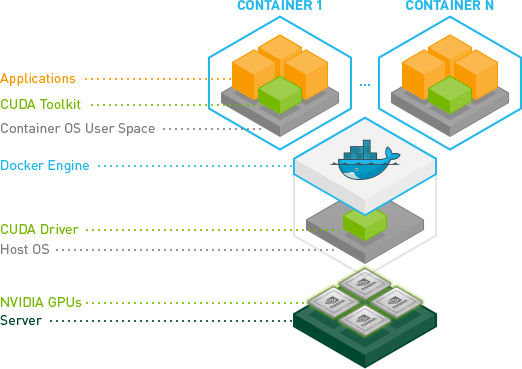
\includegraphics[width=0.6\textwidth]{MarcoTeorico/imgs/nvidia-docker.png}
    \caption{Arquitectura de Nvidia Docker \cite{nvidiaDocker2021overview}.}
    \label{fig:nvidiaDocker}
\end{figure}

